\noindent
\begin{exerciseS}[Strato limite di Blasius e sforzo a parete]
Partendo dalle equazioni di Prandtl per lo strato limite bidimensionale stazionario laminare, ricavare l'equazione di Blasius per lo strato limite laminare e le condizioni al contorno per la corrente di stato limite su una lamina semi-infinita. \newline
Ricavare poi l'espresisone dello sforzo viscoso a parete e gli spessori integrali di spostamento $\delta^*$ e di quantità di moto $\theta$. \newline
Infine, ricavare la soluzione dell'equazione di Blasius con un metodo numerico.
\end{exerciseS}

\sol

\partone Equazioni di Prandtl. Equazione di Blasius. Soluzione in similitudine. 
Shooting method.

\parttwo 

\paragraph{Dalle equazioni di Prandtl al modello di Blasius.}
Le equazioni di Prandtl dello strato limite possono essere ricavate tramite un'analisi degli ordini di grandezza delle quantità fisiche che compaiono nelle equazioni di Navier--Stokes.
%
\begin{equation}
  \begin{cases}
      u\dfrac{\partial u}{\partial x} + v\dfrac{\partial u}{\partial y} - \nu \dfrac{\partial^2 u}{\partial y^2} = - \dfrac{1}{\rho} \dfrac{d P(x)}{d x} = U(x) U'(x) \\
    \dfrac{\partial u}{\partial x} + \dfrac{\partial v}{\partial y} = 0 \ ,
  \end{cases}
\end{equation}
avendo indicato con $U(x)$ la componente parallela alla parete della lamina semi infinita del campo di velocità della corrente esterna.
Il modello di Blasius dello strato limite ipotizza che la corrente esterna sia uniforme,
%
\begin{equation}
  \begin{cases}
      u\dfrac{\partial u}{\partial x} + v\dfrac{\partial u}{\partial y} - \nu \dfrac{\partial^2 u}{\partial y^2} = 0 \\
    \dfrac{\partial u}{\partial x} + \dfrac{\partial v}{\partial y} = 0 \ .
  \end{cases}
\end{equation}
%
Si può ridurre il sistema di due equazioni nelle incognite $(u,\ v)$ a un'equazione sola in una incognita introducendo la funzione di corrente $\psi$,
\begin{equation}
 u = \partial \psi / \partial y \qquad , \qquad v = - \partial \psi / \partial x \ .
\end{equation}
Il vincolo di incomprimibilità è soddisfatto identicamente, mentre la componente $x$ dell'equazione della quantità di moto diventa
\begin{equation}
 \psi_y \psi_{yx} - \psi_x \psi_{yy} - \nu \, \psi_{yyy} = 0 \ .
\end{equation}
%
Poiché il problema non ha una scala di lunghezza, si cerca una soluzione similare. Si introduce la variabile di similitudine $\eta = y/\delta(x)$, dove $\delta(x)$ rappresenta lo spessore convenzionale dello strato limite, e si cerca la soluzione del problema imponendo l'espressione della funzione di corrente
\begin{equation}
   \psi(x,y) = U \delta(x) g(\eta(x,y)) \ .
\end{equation}
%
Utilizzando le derivate della funzione di corrente,
\begin{equation}
\begin{aligned}
    \psi_y & = U g'(\eta) \qquad , \qquad \psi_{yy} = \dfrac{U}{\delta(x)}g''(\eta) \qquad ,
    \qquad \psi_{yyy} = \dfrac{U}{\delta^2(x)}g'''(\eta) \ ,  \\
    \psi_x & = U \delta'(x) \left[ g - \eta \, g'(\eta) \right]  \qquad , \qquad
    \psi_{xy} = U \left[ - \dfrac{\delta'(x)}{\delta(x)} \, \eta \, g''(\eta) \right] \ ,
\end{aligned}
\end{equation}
all'interno dell'equazione della quantitàdi moto, si ottiene
\begin{equation}
\begin{aligned}
 & - U^2 \dfrac{\delta'}{\delta} \, \eta \, g'  g'' 
   - U^2 \dfrac{\delta'}{\delta} [ g \, g'' - \eta \, g' g'' ] - \dfrac{ \nu U }{\delta^2} g''' = 0 \ ,\\ \\
 & \qquad \qquad \qquad \rightarrow \qquad
    \dfrac{U \, \delta'(x) \delta(x)}{ \nu } g(\eta) \, g''(\eta) + g'''(\eta) = 0 \ . 
\end{aligned}
\end{equation}
Affinché la funzione $g(\eta)$ dipenda solo da $\eta(x,y)$ e non dalle due variabili $x$, $y$ in maniera indipendente, il coefficiente $U \delta'(x) \delta(x) / \nu$ deve essere uguale a una costante,
\begin{equation}
  \dfrac{U \delta'(x) \delta(x)}{ \nu } = \alpha \  .
\end{equation}
Scegliendo in maniera arbitraria $\alpha = \frac{1}{2}$ e integrando questa ultima relazione in $x$ (con condizioni al contorno $\delta(0) = 0$), si ottiene l'andamento dello spessore dello strato limite laminare di Blasius,
\begin{equation}
 \delta(x) = \sqrt{ \dfrac{ \nu x }{ U } } \ ,
\end{equation}
e l'equazione di Blasius per la funzione $g(\eta)$,
\begin{equation}
 g''' + \frac{1}{2} g g'' = 0 \ ,
\end{equation}
con le condizioni al contorno per il problema dello strato limite su lamina piana
\begin{equation}
 \begin{cases}
 g(0) = 0 \\
 g'(0) = 0 \\
 \lim_{\eta\to \infty}
 g'(\eta) = 1 \ .
 \end{cases}
\end{equation}

\paragraph{Sforzo viscoso a parete.}
La formula per lo sforzo viscoso a parete è:
\begin{equation}
  \tau_w = \mu \frac{\partial u}{\partial y}\Bigg|_{y=0} = \mu \frac{\partial^2 \psi}{\partial y^2}\Bigg|_{\eta=0} =  \mu \frac{U}{\delta(x)} g''(0) \ ,
\end{equation}
dove $g''(0) \approx 0.332$.

\paragraph{Spessori integrali dello strato limite.}
Si calcolano gli spessori integrali dello strato limite di Blasius.
%
 Usando le relazioni dello strato limite di Blasius, si trova
 \begin{equation}
 \begin{aligned}
 & \delta^* = \int_0^\infty (1 - g'(\eta(y))) dy = 
     \delta(x) \int_0^\infty (1 - g'(\eta)) d\eta \ , \\
 & \theta   = \int_0^\infty g'(\eta) (1 - g'(\eta(y))) dy = 
     \delta(x) \int_0^\infty g'(\eta) (1 - g'(\eta)) d\eta \ .
 \end{aligned}
 \end{equation}
% 
 Per lo spessore di spostamento si ha:
 \begin{equation}
 \begin{aligned}
  \delta^* & = \delta(x) \int_0^\infty (1 - g'(\eta)) d\eta = 
         & \\
           & = \delta(x) [\eta - g(\eta)]|_0^\infty = 
         & \text{($g(0) = 0$)} \\
           & = \delta(x) \lim_{\eta \to \infty} [\eta - g(\eta)] = 
         & \text{($\lim_{\eta \to \infty} [\eta - g(\eta)] = 1.721$)} \\
           & = 1.721 \cdot \delta = 
         & \text{($\delta = \sqrt{\nu x / U}$)} \\
           & = 1.721 \sqrt{\frac{\nu x}{U}} \ .
 \end{aligned}
 \end{equation}
% 
 Per lo spessore di quantità di moto:
 \begin{equation}
 \begin{aligned}
  \theta   & = \delta(x) \int_0^\infty g'(\eta) (1 - g'(\eta)) d\eta = & \\
           & = \delta \int_0^\infty g'(\eta) d\eta 
                - \delta \int_0^\infty g'^2(\eta) d\eta = & \\
           & = \delta [g(\eta)]|_0^\infty 
                - \delta \int_0^\infty g'^2(\eta) d\eta = 
         & \text{($g(0)=0$ e IxP)} \\
           & = \delta \lim_{\eta \to \infty}  g(\eta) 
                - \delta \int_0^\infty [(g g')' - g g''] d\eta = 
         & \text{(eq. di Blasius: $\frac{1}{2}g g'' + g''' = 0$)} \\
           & = \delta \lim_{\eta \to \infty}  g(\eta) 
                - \delta [g g']|_0^\infty 
                - \delta \int_0^\infty 2 g''' d\eta = 
         & \text{($g(0) = 0$)}\\
           & = \delta \lim_{\eta \to \infty}  g(\eta)
                - \delta \lim_{\eta \to \infty}  g(\eta)g'(\eta)
                - 2 \delta [g''(\eta)]|_0^\infty = 
         & \text{($\lim_{\eta \to \infty} g'(\eta) = 1$, 
           $\lim_{\eta \to \infty} g''(\eta) = 0$)} \\
           & = 2 \delta(x) g''(0) = \\
           & = 0.664 \sqrt{\frac{\nu x}{U}} \ .
 \end{aligned}
 \end{equation}
% 
 Il rapporto di forma vale quindi $H = \delta^* / \theta = 1.721 / 0.664$, cioè
 $H = 2.59$.

% --------------
 \begin{figure*}[h!]
 \centering
   \subfloat[]
     [\emph Grafico di $g(\eta)$: per $\eta \to \infty$ g ha derivata uguale a $1$; l'intersezione dell'asintoto con l'asse orizzontale avviene per $g(0)=1.721$: $g(\eta) \sim \eta - 1.721$ per $\eta \rightarrow \infty$.]
     {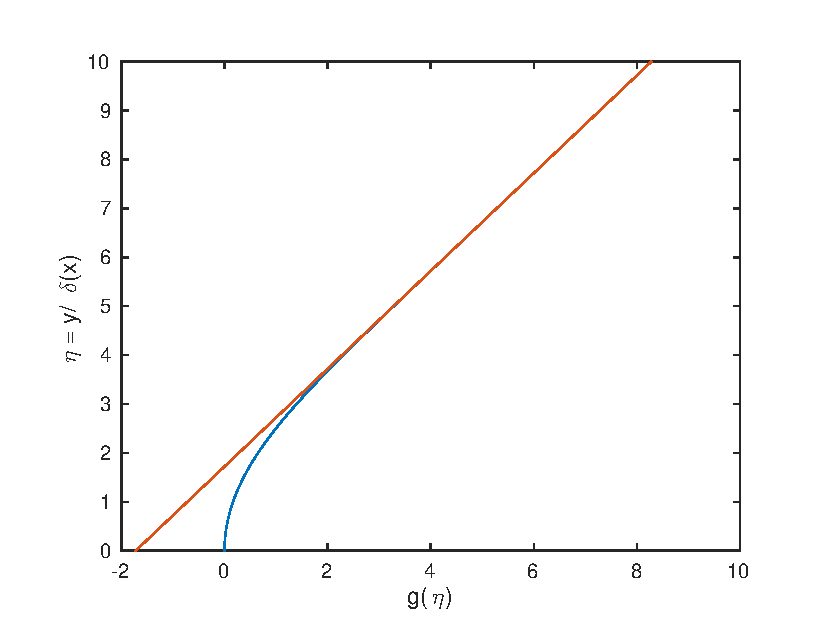
\includegraphics[width=.31\textwidth]{./fig/BlasiusShooting/g.eps}} \quad
   \subfloat[]
   [\emph Grafico di  $g'(\eta)$: rappresenta il profilo adimensionale dela velocità. Per
   $\eta \to \infty$ $g'(\eta) \to 1$.]
     {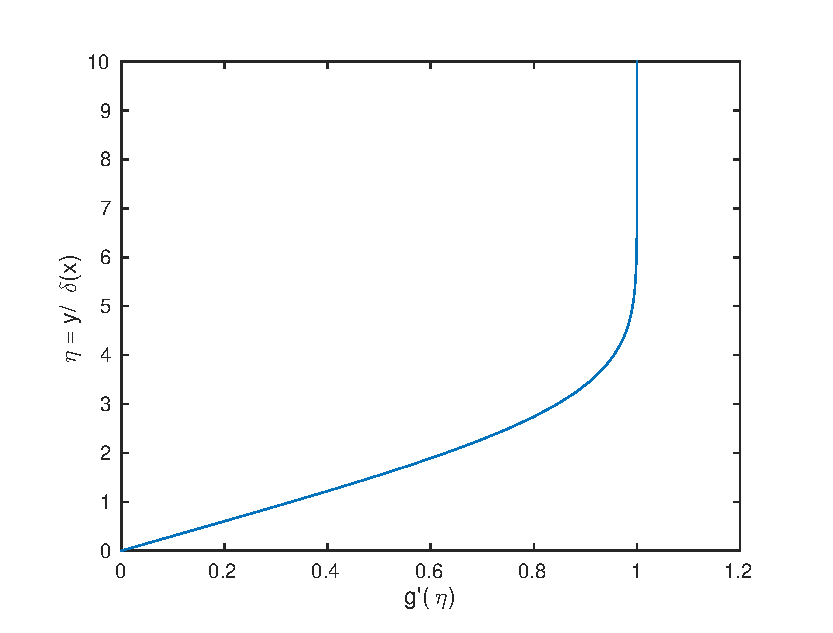
\includegraphics[width=.31\textwidth]{./fig/BlasiusShooting/dg.eps}} \quad
   \subfloat[]
   [\emph Grafico di $g''(\eta)$: è legato alla derivata parziale $\partial u / \partial y$. 
   Per determinare lo sforzo a parete è necessario trovare il valore di $g''(0)$: $g''(0) = 0.332$]
     {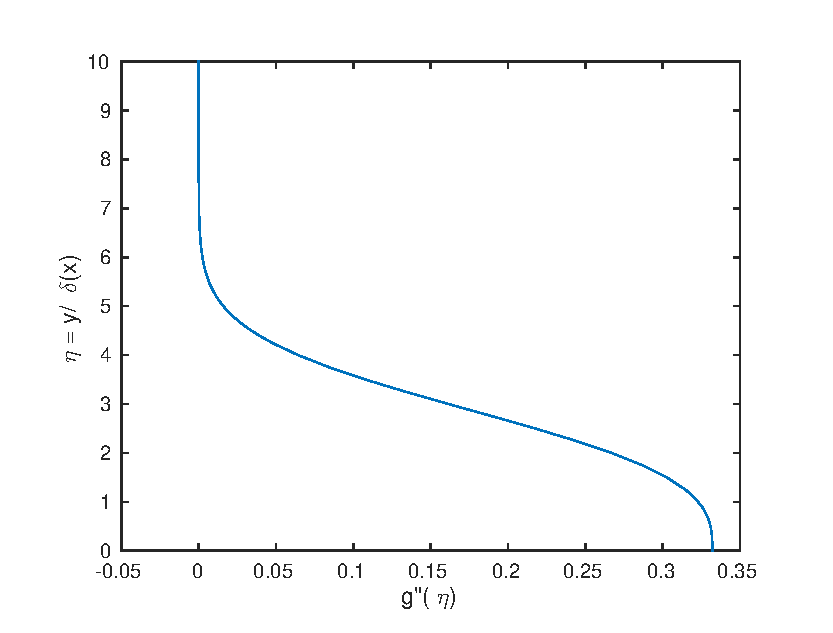
\includegraphics[width=.31\textwidth]{./fig/BlasiusShooting/ddg.eps}}
\end{figure*}

\paragraph{Soluzione numerica: shooting method.}
Per risolvere l'equazione di Blasius con metodi numerici, si può incontrare qualche difficoltà
nell'imporre la condizione al contorno per $\eta \to \infty$.
Tramite uno \textit{shooting method} si può risolvere il problema ai valori al contorno, tramite 
la soluzione di problemi ai valori iniziali insieme a un metodo per trovare gli zeri di una
funzione (es. Newton).
Il dominio semi-infinito viene troncato. Il dominio numerico è quindi $[0,\bar{\eta}]$. L'equazione 
scalare di terzo ordine, viene scritta come sistema del primo ordine. Invece di imporre la condizione
all'infinito, viene imposto il valore di $g''(0)=\alpha$. Si risolve l'equazione. Si trova il valore di $g'_n$in $\bar{\eta}$.
Si itera fino a quando il valore assoluto di $F(\alpha) = g'_n(\bar{\eta};\alpha) - \lim_{\eta\to \infty} g'(\eta)$ non è inferiore 
a una tolleranza stabilita.
%
Per esempio, partendo da $\alpha=0.1$, con una tolleranza $tol = 1E-09$:
\begin{center}
\begin{verbatim}
nIter    g"(0)    res 
  1     0.1000  5.508e-01 
  2     0.2836  9.975e-02 
  3     0.3308  2.575e-03 
  4     0.3320  1.660e-06 
  5     0.3320  1.804e-12
\end{verbatim}
\end{center}
    


